\documentclass{article}

\usepackage[utf8]{inputenc}
\usepackage{amsmath}
\usepackage{amssymb}
\usepackage{anysize}
\usepackage{color}
\usepackage{xcolor}
\usepackage{graphicx}
\usepackage{float}


\newcommand{\BigO}[1]{\ensuremath{\operatorname{O}\bigl(#1\bigr)}}

\usepackage{listings}
\lstset{
	language=C++,                	% choose the language of the code
	basicstyle=\footnotesize,       % the size of the fonts that are used for the code
	numbers= left,                 	% where to put the line-numbers
	numberstyle=\footnotesize,      % the size of the fonts that are used for the line-numbers
	stepnumber=1,                   % the step between two line-numbers. If it is 1 each line will be numbered
	numbersep=5pt,                  % how far the line-numbers are from the code
	backgroundcolor=\color{white},  % choose the background color. You must add \usepackage{color}
	showspaces=false,               % show spaces adding particular underscores
	showstringspaces=false,         % underline spaces within strings
	showtabs=false,                 % show tabs within strings adding particular underscores
	frame=single,           		% adds a frame around the code
	tabsize=2,          			% sets default tabsize to 2 spaces
	captionpos=t,          			% sets the caption-position to bottom (t=top, b=bottom)
	breaklines=true,        		% sets automatic line breaking
	breakatwhitespace=false,    	% sets if automatic breaks should only happen at whitespace
	escapeinside={\%*}{*)}          % if you want to add a comment within your code
}



\usepackage{caption}
\DeclareCaptionFont{white}{\color{white}}
\DeclareCaptionFormat{listing}{\colorbox{gray}{\parbox[c]{\textwidth}{#1#2#3}}}
\captionsetup[lstlisting]{format=listing,labelfont=white,textfont=white}

\setlength\parindent{0pt}
\setlength{\parskip}{10pt}

\marginsize{3cm}{2cm}{2cm}{2cm}

\title{Sensors and Digitization\\
		Moving Object Imaging\\
		Lab 1 Report\\
		GrTP1A}
\author{Daniel Sileshi Asfaw\\
		Emre Ozan Alkan\\}
\date{4 December 2013}

\begin{document}
\maketitle

\section{Introduction}
	\subsection{Objective}
	The main goal was to understand how a simple camera can be transformed into a polarization state measurement system. This lab introduces two different systems:
	\begin{enumerate}
	\item A simplified polarization imaging set-up that consist of a manually rotating polarizer placed in front of the sensor.
	\item A contrast polarization measurement system that uses a Twisted Nematic Liquid crystal.
	\end{enumerate}

	\subsection{Equipment}
	In the lab room, we had following equipment to use:
	\begin{itemize}
		\item PC Computer
		\item Frame Grabber - IEEE 1394
		\item Camera - Allied Vision Technologies GUPPY + one lens + Video Cable
		\item Arcoptix switchable polarization rotator 0-90 degree (Twisted Nematic Liquid Crystal) + Arcoptix USB LC Driver
		\item Two linear polarizers
		\item Four mounting posts and four post holders
		\item Lighting Device + Polarized Ring
	\end{itemize}		
	
	\subsection{Software}
	We used the following software in the lab computers:
	\begin{itemize}
		\item National Instruments "Measurement \& Automation Explorer" Software
		\item Arcoptix USB LC Software
		\item Matlab or National Instruments LabVIEW
	\end{itemize}
	
	In this laboratory, we performed three different experiments; the first experiment was grabbing images using one linear polarizer, the second was contrast polarization measurement using two linear polarizer also we have experimented using liquid crystal polarizer on the middle of the two linear polarizer, the last experiment was to study one application of polarization, diffuse specular reflection.
	
	
\section{Simplified Polarization Imaging}	
	\subsection{Wolffs Method}
	\begin{figure}[H]
	\centering
	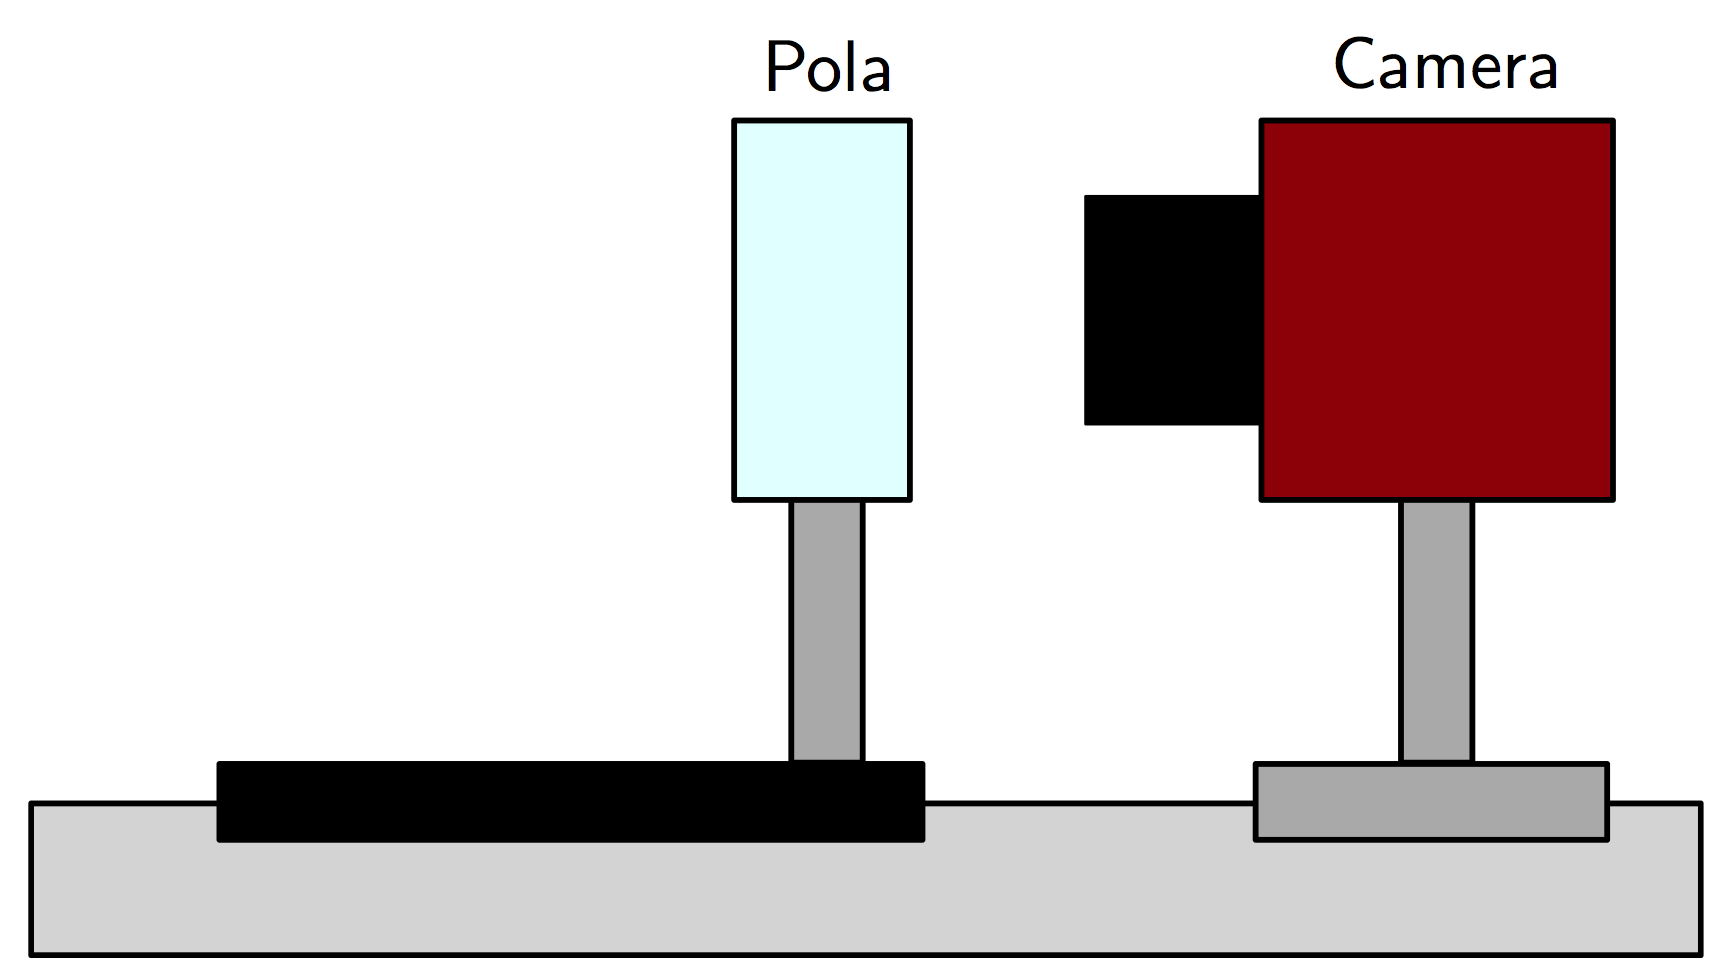
\includegraphics[scale=0.2]{polaSetup1.png}
	\caption{First Setup}
	\end{figure}
	We first setup all these imaging equipment as in figure [1]. We adjusted the camera position will capture computer screen as a part of the grabbing scene. In order to avoid reflection seen from appearing on the graded image we position the camera as close as possible to the polarizer.
The "Measurement \& Automation Explorer" Software is opened to start grabbing an image. We start grabbing an image by changing the angle of the polarizer. From the grabbed image we observe that the computer screen's contrast value was caning while we were changing the angle of the polarizer. The reason of this phenomenon is that computer screen is already polarized.

	Here is the image grabbed with different polarizer orientations(0, 45 and 90 degrees)
	\begin{figure}[H]
	\centering
	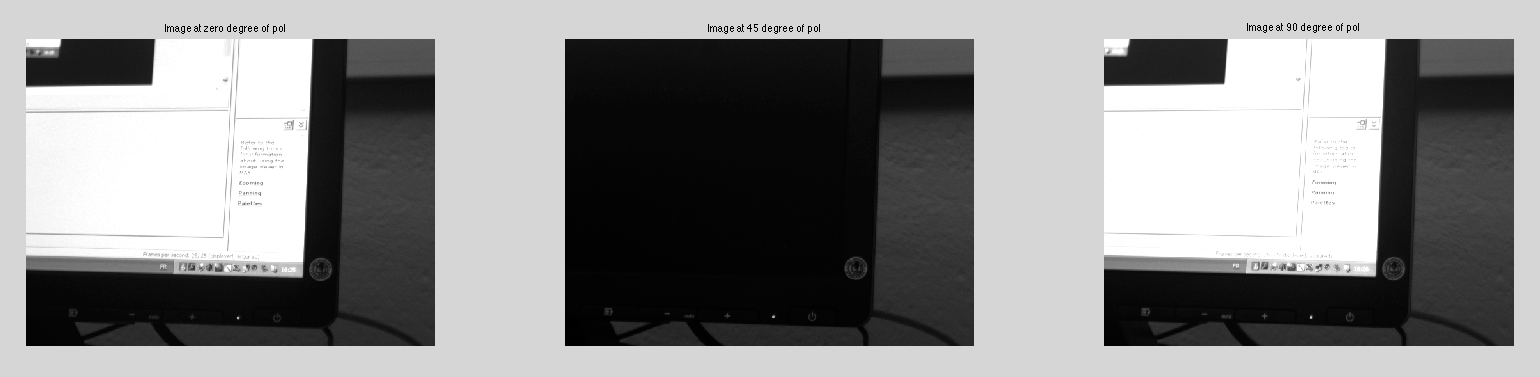
\includegraphics[scale=0.32]{PolaFirstPartImage1.png}
	\caption{0 - 45 - 90}
	\end{figure}
	
	We used MATLAB to calculate the special case of least mean square method (Wolff's method) to find the following parameters through three grabbed images as in equation below:
	\begin{figure}[H]
	\centering
	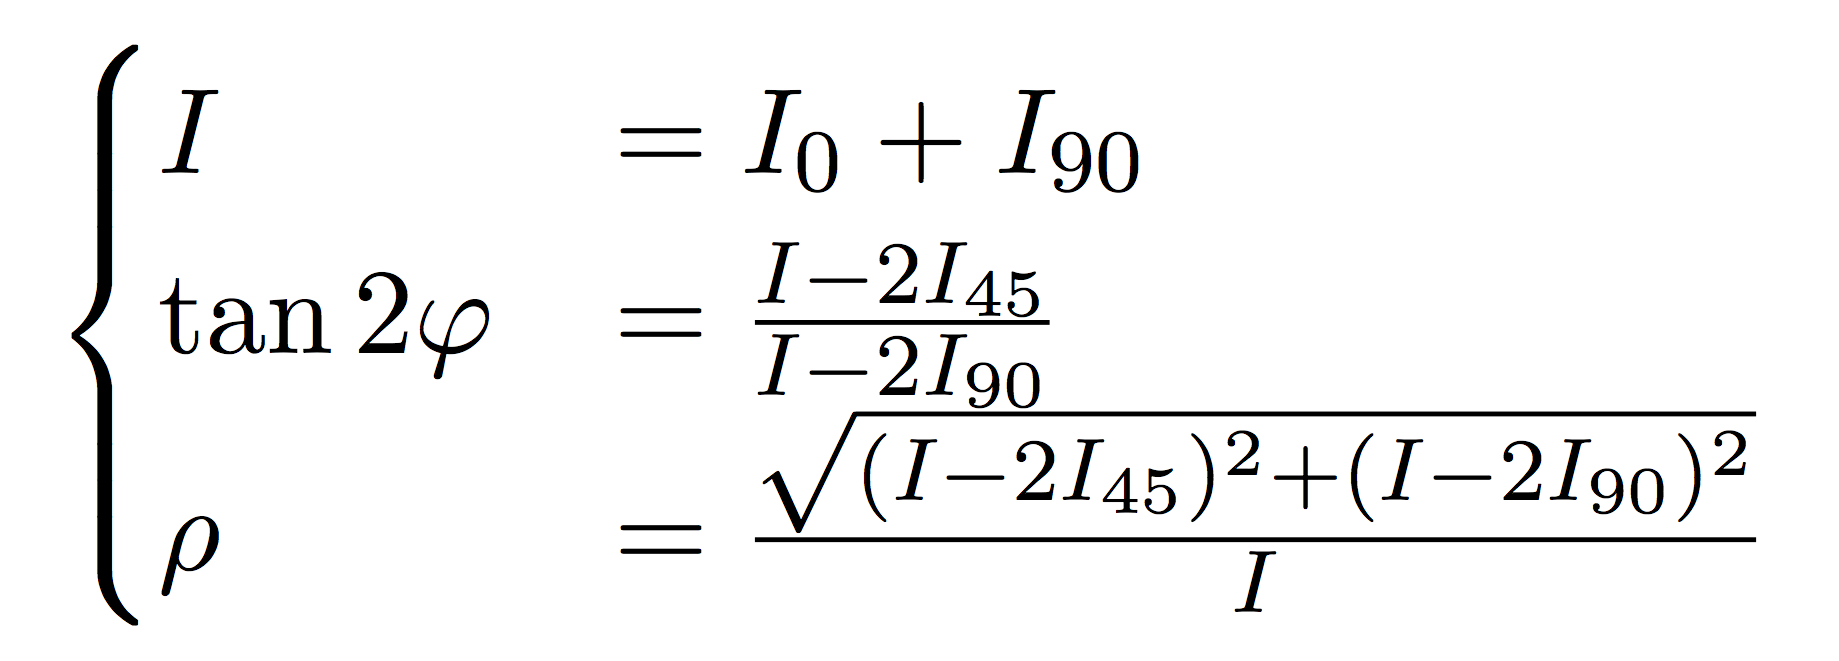
\includegraphics[scale=0.1]{WolffMethod.png}
	\caption{Wolff's Method}
	\end{figure}
	
	Those three values are HSV color image representation of the image. Where H is angle of polarization S is degree of polarization and V is the intensity.
	\begin{figure}[H]
	\centering
	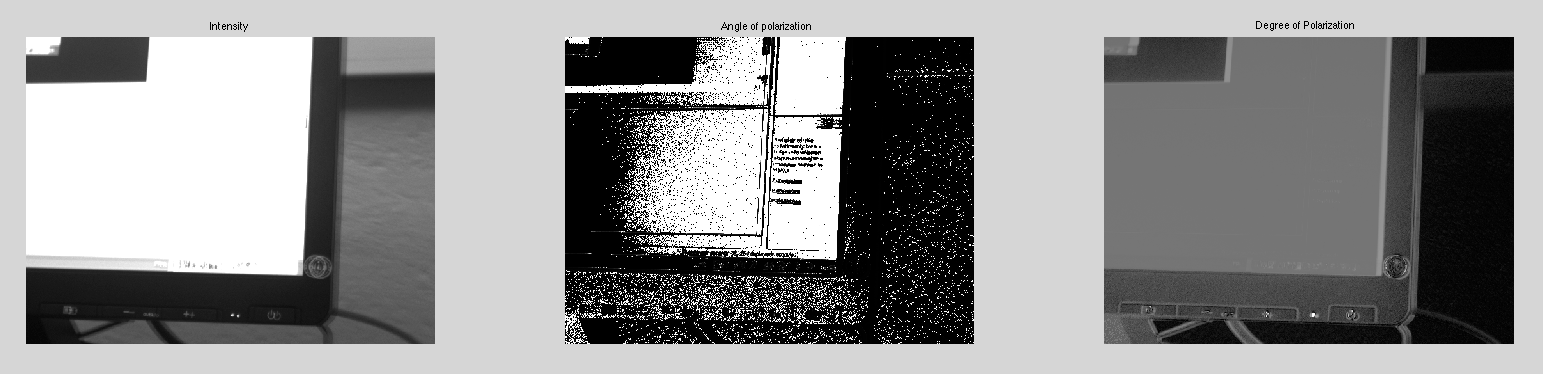
\includegraphics[scale=0.30]{PolaFirstPartImage2.png}
	\caption{Wolff's Method Gray Scale Results}
	\end{figure}
	
	\begin{figure}[H]
	\centering
	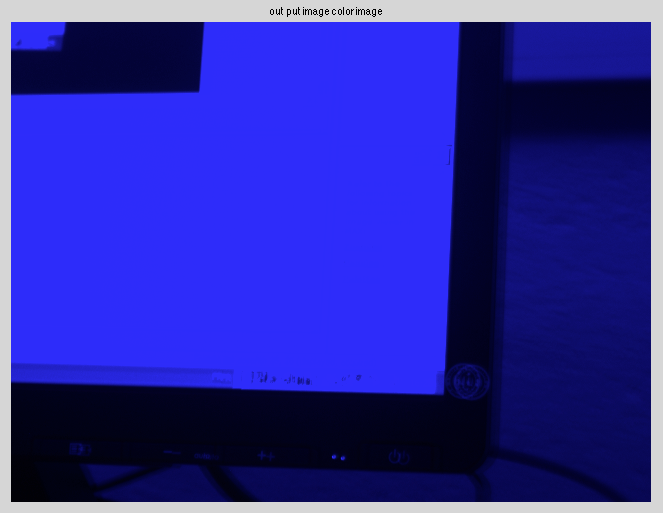
\includegraphics[scale=0.2]{PolaFirstPartImage3.png}
	\caption{Wolff's Method HSV Result}
	\end{figure}
	
	\subsection{Least Mean Square Method}
	We took 8 photos with degrees 0, 45, 90, 135, 180, 225, 270, 315, respectively:
	\begin{figure}[H]
	\centering
	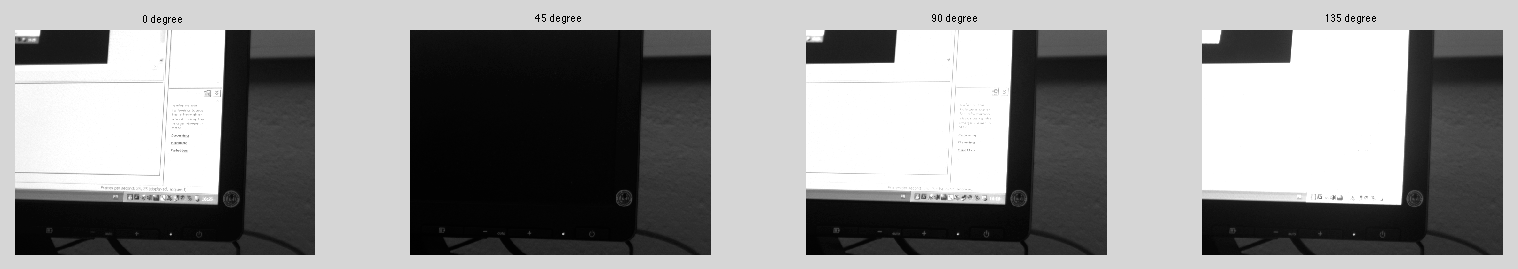
\includegraphics[scale=0.33]{LMSM1.png}
	%\caption{Wolff's Method HSV Result}
	\end{figure}
	\begin{figure}[H]
	\centering
	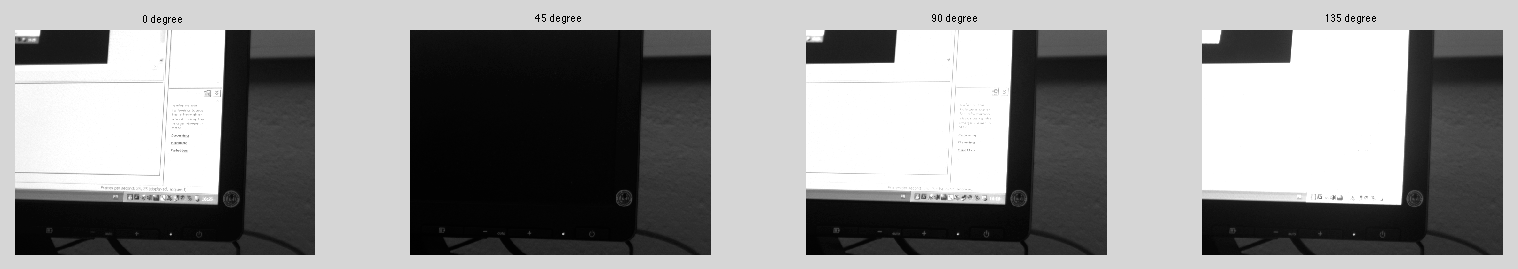
\includegraphics[scale=0.33]{LMSM1.png}
	%\caption{Wolff's Method HSV Result}
	\end{figure}
	
	Then we applied Least Mean Square Method for images as we seen in class. Here is the results:
	\begin{figure}[H]
	\centering
	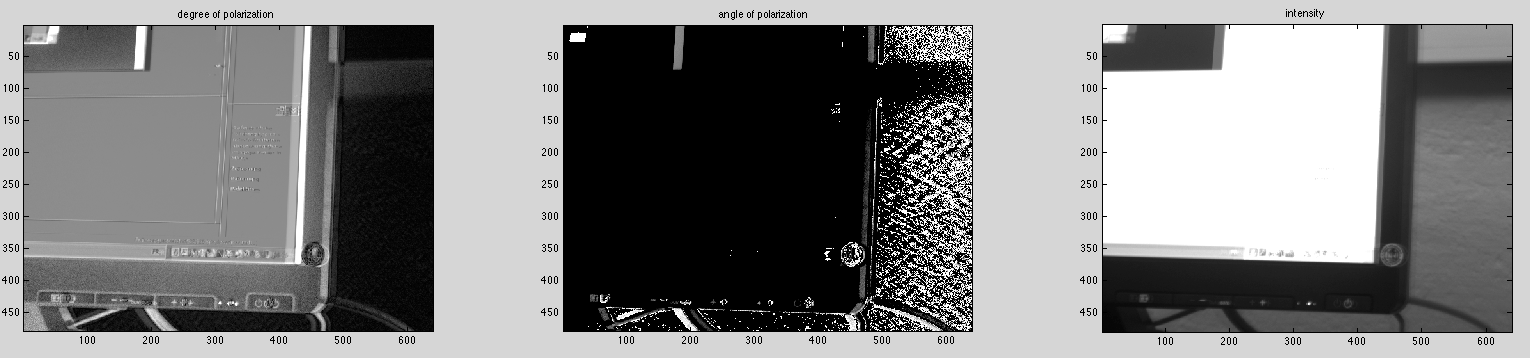
\includegraphics[scale=0.33]{LMSMResult.png}
	\caption{Least Mean Square Method Result}
	\end{figure}
	
	And here is the sinusoidal relationship of the images:
	\begin{figure}[H]
	\centering
	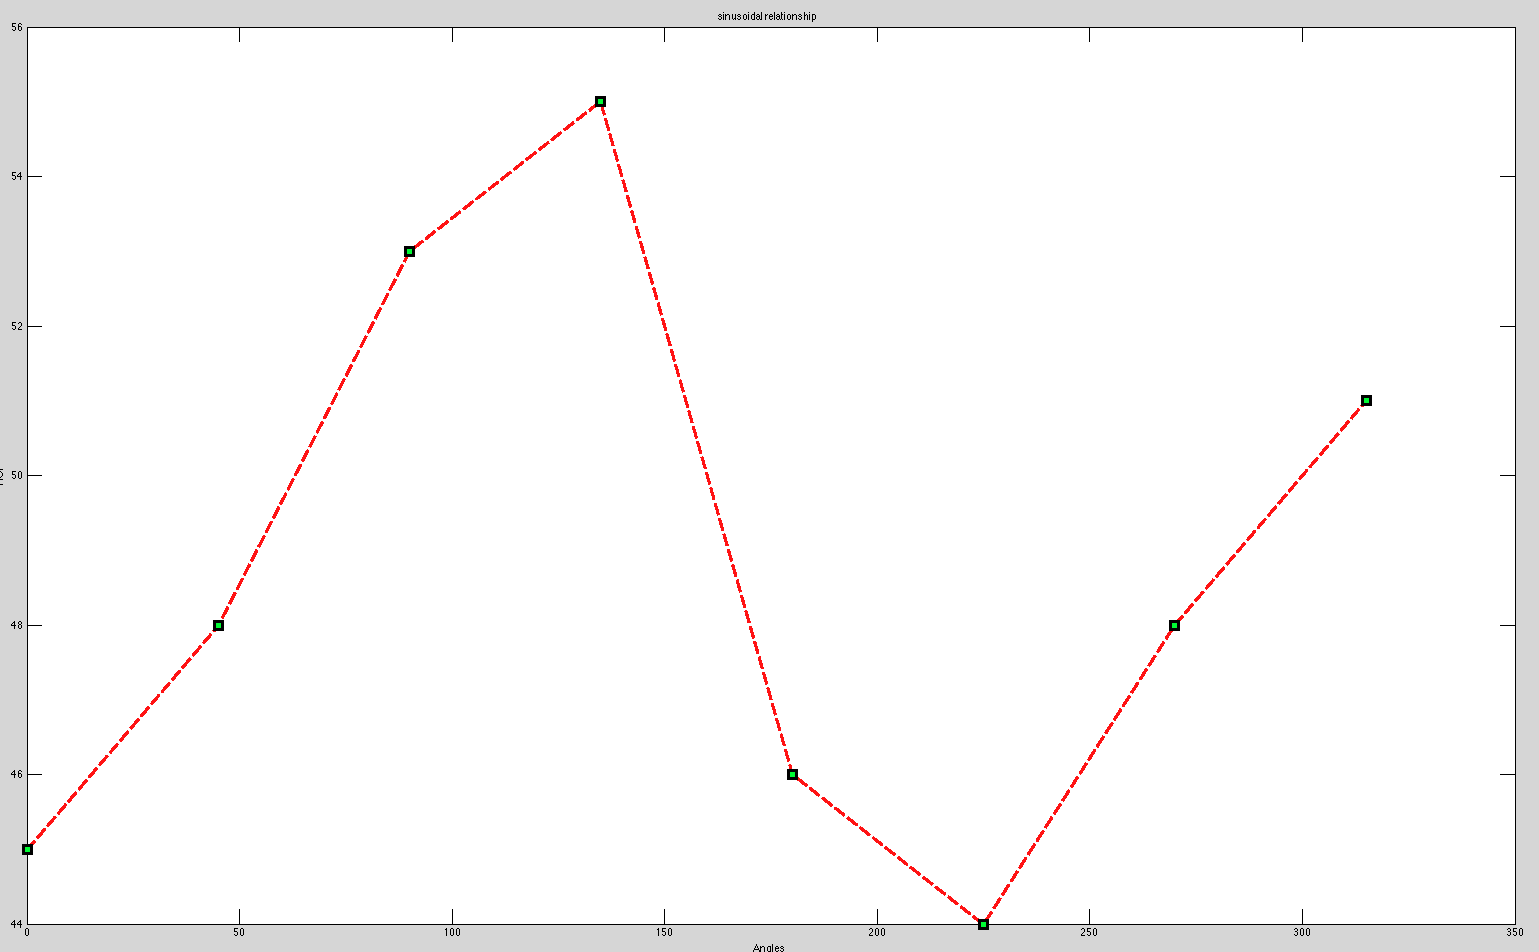
\includegraphics[scale=0.3]{LMSMSinusoidalRelationship.png}
	\caption{Least Mean Square Method Sinusoidal Relationship}
	\end{figure}
	
	
	
	
\section{Contrast polarization measurement}

	\subsection{2 Linear Polarizers}
	\begin{figure}[H]
	\centering
	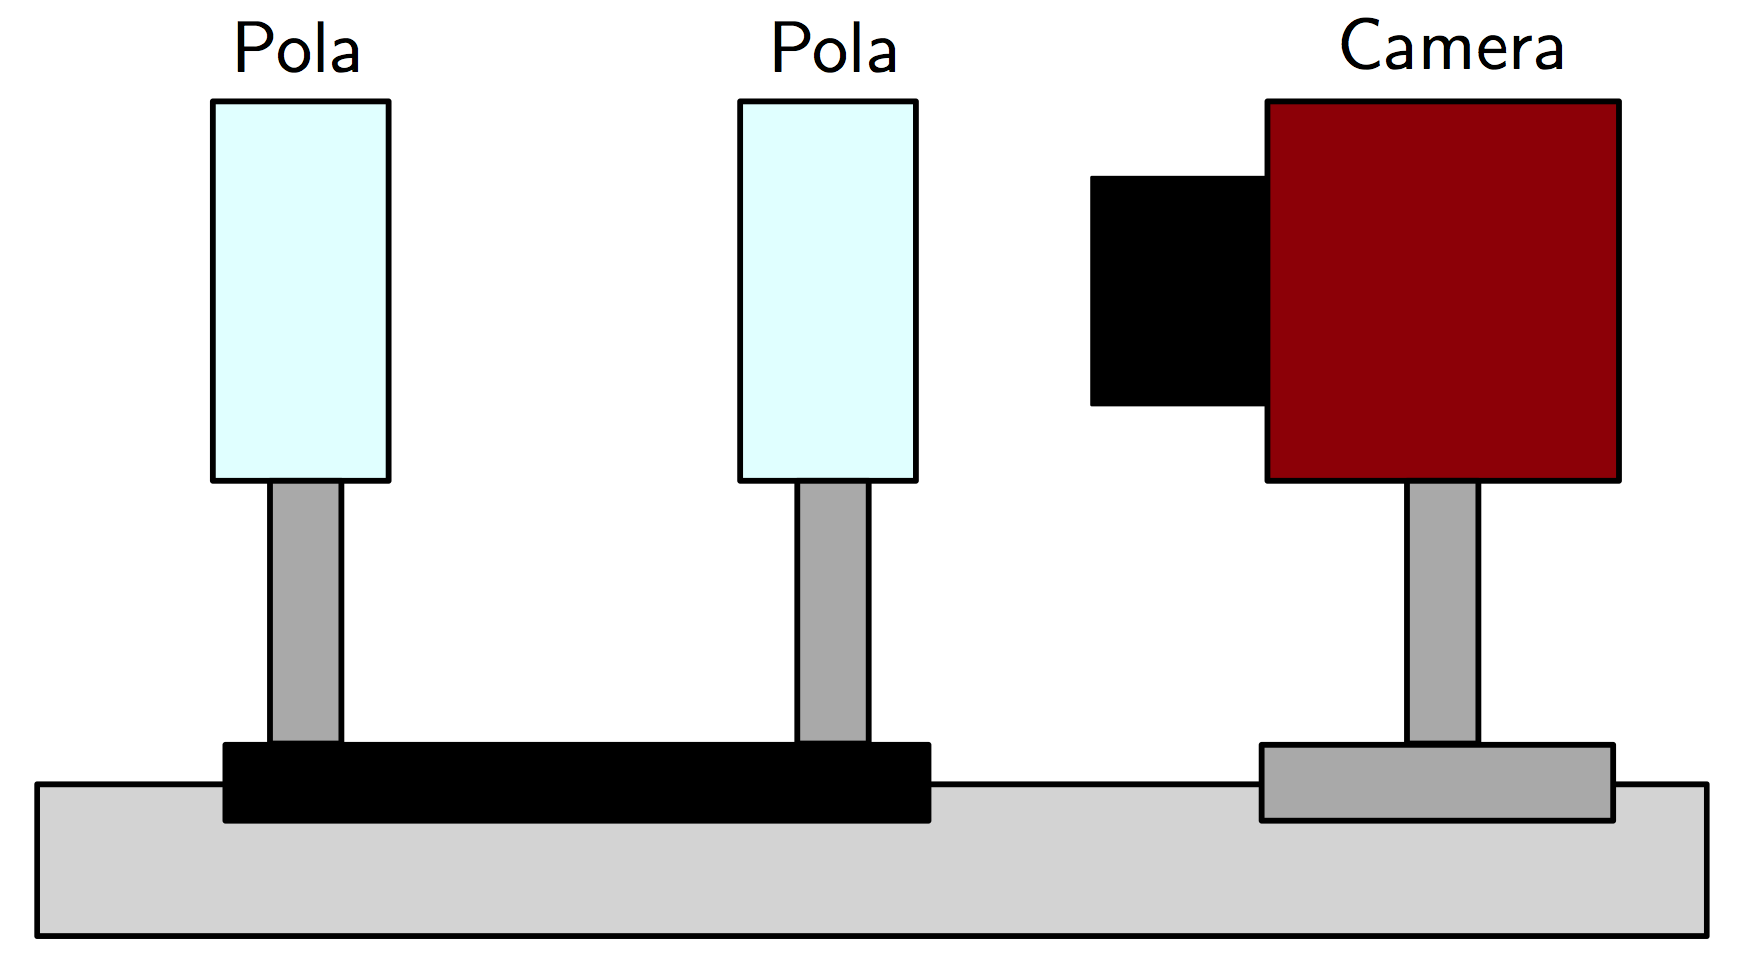
\includegraphics[scale=0.2]{polaSetup2.png}
	\caption{2 Linear Polarizer Setup}
	\end{figure}
	We setup all the imaging equipment as in figure above. We start by adjusting polarization angle to of the two linear polarizer to zero. We observed that output image is darker but more readable than one from first experiment at same orientation using a single polarizer. Also intensity decreased a lot because we using 2 polarizer as a result of malus' law.
	
	
	
	
	
	\subsection{Introducing Liquid Crystal}
	\begin{figure}[H]
	\centering
	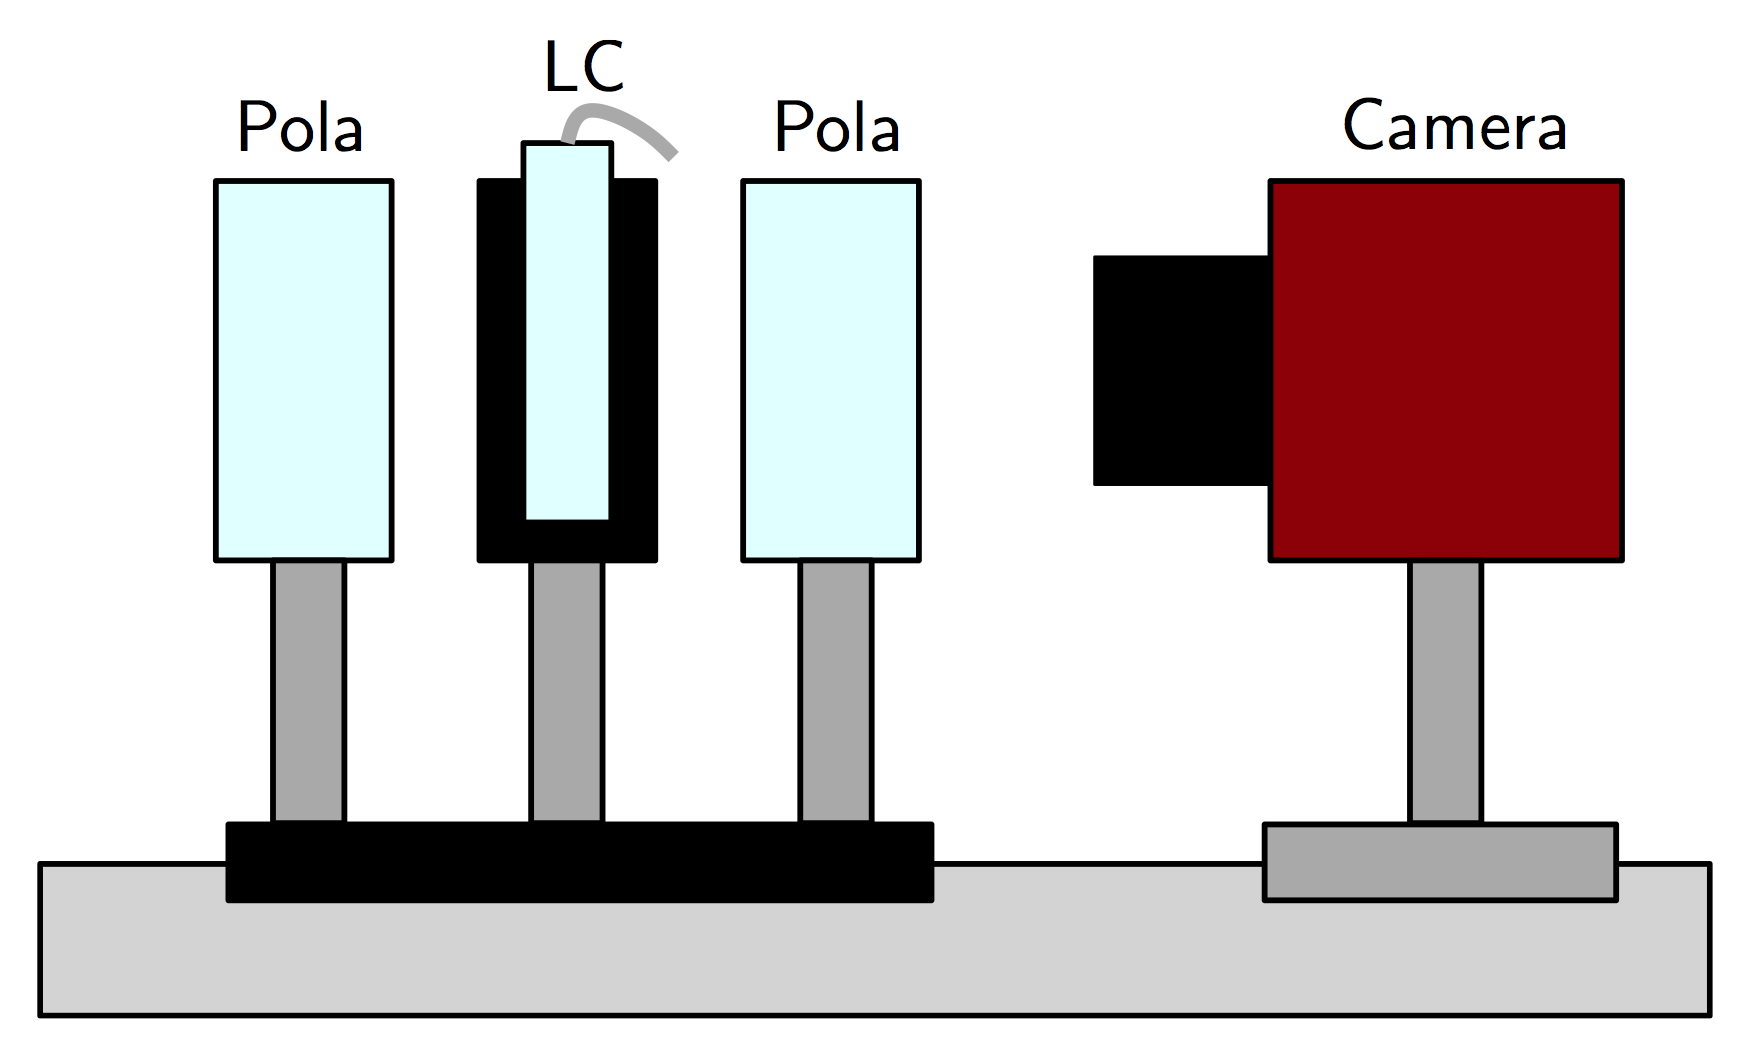
\includegraphics[scale=0.2]{polaSetup3.png}
	\caption{Introducing Liquid Crystal}
	\end{figure}
	The liquid crystal is put between the polarizer. This switchable polarization rotator works  by controlling the amount input voltage using Arcoptix software. It works in binary mode. It rotates to 90 degree when input voltage is applied and zero degree when input voltage is 0V.This set up helps to automate the rotation when experimenting effect of polarization using two linear polarizers.
	
	
	
	\subsection{Diffuse Specular Reflection}
	\begin{figure}[H]
	\centering
	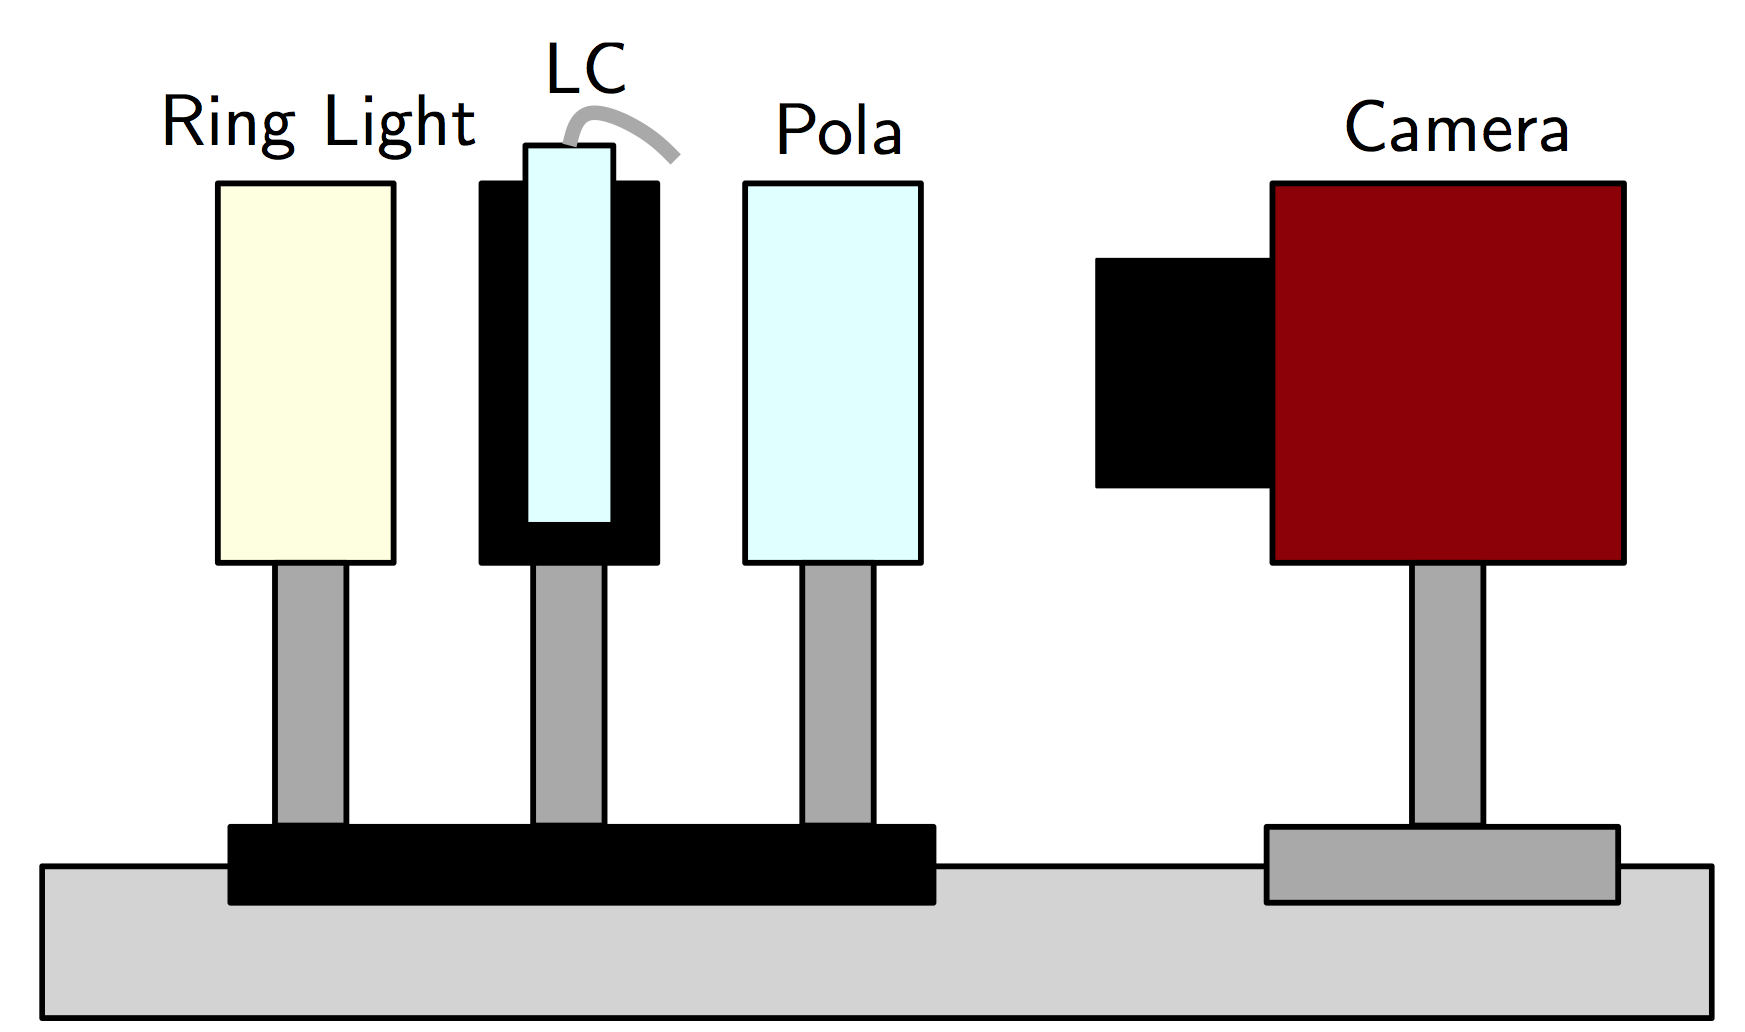
\includegraphics[scale=0.2]{polaSetup4.png}
	\caption{Using Polarized Lighting Source}
	\end{figure}
	We setup all the imaging equipment as in figure above by putting Polarized Ring with Lighting Device in front of the polarizers. And we started snapping two different images of two different objects (hand and metal object) at two different polarization angles (0 and 90 degrees).
	\begin{figure}[H]
	\centering
	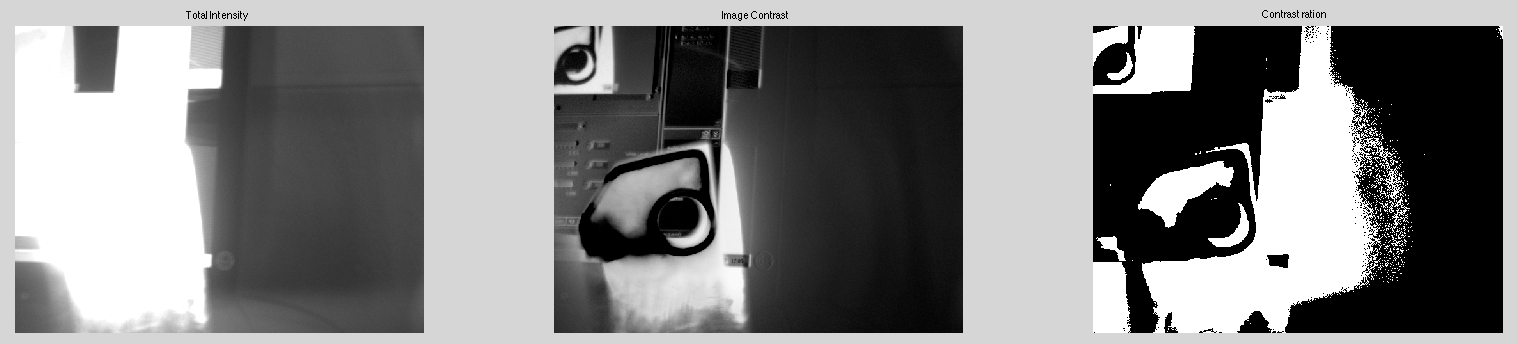
\includegraphics[scale=0.32]{diffuseSpecularReaction.png}
	\caption{Removing Specular Reflection}
	\end{figure}
	
We observed that specular reflection (smooth or shiny surface of an object) can be removed by setting the polarization rotator to 0V (shiny metal example), but diffuse reflection like hand, can’t be removed at any setting.


\section{MATLAB CODES}
	\subsection{Wolffs Method}
	
	\begin{lstlisting}[label=exercices-h-traversal,caption=Wolffs]	

image_zero = imread('0.png');
I_0 = double(image_zero);

image_45 = imread('45.png');
I_45 = double(image_45);

image_90 = imread('90.png');
I_90 = double(image_90);
%============= Wolff's method ==============
%intiallize the out put images to zero first
I = zeros(size(I_0));
Phi = zeros(size(I_0));
Ro = zeros(size(I_0));

for i=1:size(I_0,1)
    for j=1:size(I_0,2)
        for k=1:size(I_0,3)
            I(i,j,k) = I_0(i,j,k) + I_90(i,j,k);
            Phi(i,j,k) = (((I(i,j,k)-2*I_45(i,j,k))/(I(i,j,k)-2*I_90(i,j,k))));
            Ro(i,j,k) = (sqrt(((I(i,j,k)-2*I_45(i,j,k)).^2) + ((I(i,j,k)-2*I_90(i,j,k)).^2))/I(i,j,k));
        end
    end
end



%create the 3D color image by concating the above three results and
%display the image
Image_out = uint8(cat(3,atan(Phi),Ro,I));%this image is hsv image 

figure,subplot(131), imshow(image_zero);title('Image at zero degree of pol');
subplot(132),imshow(image_45);title('Image at 45 degree of pol');
subplot(133),imshow(image_90);title('Image at 90 degree of pol');

 figure (2),subplot(131), imshow(uint8(I));title('Intensity');
 subplot(132),imshow(uint8((Phi)));title('Angle of polarization');
 subplot(133),imshow(uint8(Ro*100));title('Degree of Polarization');
 figure(3), imshow(Image_out);colormap(hsv);title('out put image color image');
 
	\end{lstlisting}
	
	\subsection{Least Mean Square Method}
	
		\begin{lstlisting}[label=exercices-h-traversal,caption=Least Mean Square Method]	
Im(1,:,:) = double(imread('0.png'));
Im(2,:,:) = double(imread('45.png'));
Im(3,:,:) = double(imread('90.png'));
Im(4,:,:) = double(imread('135.png'));
Im(5,:,:) = double(imread('180.png'));
Im(6,:,:)= double(imread('225.png'));
Im(7,:,:)= double(imread('270.png'));
Im(8,:,:) = double(imread('315.png'));

image_zero = imread('0.png');
Im_0 = double(image_zero);

[m n] = size(Im_0);


Im_out = zeros(m,n,3);
for i=1:m
for j=1:n
A = [];
Y = [];
for k=1:8 
    
A = [ A; 1 cos(2*k*45) sin(2*k*45) ];
Y =  [Y ;Im(k,i,j)];

end

X = 2 .* (inv(A' * A)) * (A' * Y);
I = X(1);
Ro = sqrt(X(2).^2 + X(3).^2) ./ X(1);
Phi = atan(X(3) ./ X(2));
Im_out(i,j,:) = [ I Ro Phi];
end
end

figure(6);subplot(131); subimage(Im_out(:,:,2));  title('degree of polarization');
subplot(132); subimage(Im_out(:,:,3));  title('angle of polarization');
subplot(133); subimage((uint8(Im_out(:,:,1)))); title('intensity');

% Sinusodial Relationship
yaxis=[Im_0(162,520) Im_45(162,520) Im_90(162,520) Im_135(162,520) Im_180(162,520) Im_225(162,520) Im_270(162,520) Im_315(162,520)];
xaxis = [0 45 90 135 180 225 270 315];
figure(5);plot(xaxis,yaxis,'--rs','LineWidth',2,...
                'MarkerEdgeColor','k',...
                'MarkerFaceColor','g',...
                'MarkerSize',10);
title('sinusoidal relationship');
xlabel('Angles');
ylabel('ROI');
		\end{lstlisting}
	



	
	
	
	
	
	
	\subsection{Diffuse Specular Reflection}
	
		\begin{lstlisting}[label=exercices-h-traversal,caption=Specular Reflection Removal]
% Diffuse Specular reflection
parell = imread('Metal_0V.png');
Orto = imread('Metal_1V.png');

Total_Intensity = parell + Orto;
Contrast = parell - Orto;
Contrast_ratio = Contrast./Total_Intensity;


subplot(1, 3, 1), imshow(uint8(Total_Intensity));colormap(gray); title('Total Intensity');
subplot(1, 3, 2), imshow(uint8(Contrast));colormap(gray);title('Image Contrast');
subplot(1, 3, 3), imshow(uint8(Contrast_ratio), []);colormap(gray);title('Contrast ration');
		\end{lstlisting}
	
	
	
	
	
	
	
	
	

	
	
	
	
	
	
	

\end{document}
